\chapter{Dark matter}

\stracka{sui dialoghi ne riparliamo. Leggo prima con calma. Come prima reazione
direi di lasciarli a Galileo (che ha passato i suoi guai), ma l'ora è tarda, e
quindi domani potrei avere cambiato idea. L'importante è che eviti di dare
l'impressione di aver masticato peyote.}

\stracka{Secondo me il dialoghetto potrebbe stare in un prologo, una specie di
cap. 0 separato dal cap.1. Sentiamo che ne dirà Eugenio.
%
Cmq credo che alcune conclusioni siano un po' avventurose. Ad esempio: è vero
che hai informazioni sulla possibile distribuzione della DM, ma cosa ti porta a
escludere che \emph{tutta}
 la DM sia distribuita così? Es., non ci potrebbero essere
più componenti di DM?
%
In quel caso, dire che un modello di DM non permette di giustificare la DM (o
una sua frazione consistente) non è equivalente a dire che è stata esclusa la
presenza di un tipo di DM che si comporta così.}

When introducing the subject of fluid dynamics, one starts by considering an
ideal fluid with indefinite extension, that sits alone in the universe, has no
particular properties, does not undergo chemical reactions, has no friction,
and is subject only to forces with an easy to write expression, such that the
kinetic equation can be exemplified without too much fuss. This spherical cow
fluid does not know the beauty of the foam riding on sea waves, of violent
explosions, of sinking treasures, of stars shining with the power of a million
suns, nor anything that makes fluids interesting in real life. I consider it a
great victory of Physics that most of the matter in the universe is indeed such
a fluid.

While preparing the work for this thesis, I had the occasion to talk to a
friend I had not seen in a while. He is endowed with a rather curious mind, so
he gladly listened to me talking about dark matter. After I explained that the
visible part of the Milky Way is overlapped with an invisible halo of an
intangible substance that is probably passing through us at every instant, he
immediately asked if this ``dark galaxy'' has solar systems, planets, life,
a complete world parallel to ours.

<<Of course \emph{you} would ask such a question!---I replied---And, of course,
the answer is \emph{no}.>> I continued: <<Dark matter has no friction, it can
not agglomerate to form objects. We know this because from the gravitational
attraction exerted by the dark matter halo we can infer its shape, and it is
spherical, while the galaxy is a disc with a central bulge. Now if you think
about it, all the structure of the galaxy is recursively a ball surrounded by a
disc: the solar systems are like that, and each planet in turn can have
satellites and rings, then you can even have stuff orbiting around satellites,
and then your weird hat.>>

<<Yes\ldots>>

<<If the planets are not sufficiently discous for you, consider the asteroid
belt, and that the planets originated from a more homogeneous disk of matter
swirling around the sun. This is not a coincidence, because nothing is ever a
coincidence. This fractal pattern originates from the effect of friction, and
the conservation of angular momentum.>>

<<You have to breathe, Giacomo.>>

<<\emph{gasp}---You know what happens when a ballerina closes her arms, right?
She spins faster. Now imagine a primordial, immense, uniform sphere of matter
standing still. It will start collapsing under the effect of the gravitational
force. This is a \emph{really} vast sphere, so as it contracts the radius can
reduce by a large factor before it arrives at the scale of the galaxy. Now, if
there is even just a slight perturbation to the initial stillness of the
sphere, at some point in the contraction this turns into a significant
rotational speed, which grows continuously. Do you know what happens to
something that rotates too fast?>>

<<Sigh. It feels sick?>>

<<It \emph{breaks down}. The external shell of the sphere gets thrown around in
shards, while the core, freed from the faster rotating parts, can continue
shrinking. This process can repeat until the inner core is small enough that
the pressure of the compressed matter starts balancing the gravitational force.
So now you have a core surrounded by a large spherical cloud of matter
streaming around it. This is still spherical, because things that break are
chaotic, but the only possible final outcome is that it forms a disk. This is
because the way of preserving the angular momentum that minimizes the kinetic
energy is by just performing the rotation implied by the momentum, without
additional directions of movement. Since friction dissipates energy, with time
the sphere will flatten into a disc.>>

<<\ldots>>

<<A more direct way to picture this is the following: consider each lump of
matter orbiting around chaotically in the cloud. They go in different
directions, so the pieces will regularly cross and knock each other. This is a
sort of battle between different orbital planes. What plane will prevail in the
end? The only one that, even if alone, would be able to preserve the angular
momentum. In principle friction can collapse the disc too, but it is much
slower because there are no hard hits, the only friction is a smooth one
between the concentric layers of the disc that rotate at different speeds. And,
when the disk is steady, each part of this thing that now looks more like a
galaxy will start collapsing on its own, since it is not perturbed any more.
Once the pieces have collapsed they do not touch each other, and so the global
shape is frozen. The local collapses produce stars, and so on until satellites.
The process stops because small things are too solid---friction wins over
gravity. Matter piles up and can not shrink any more.

Now, what happens if there is no friction? Let me answer for you. The answer is
not that we get sub-planets and sub-satellites and tiny sub-hats. Go back to
the beginning. The primordial sphere is collapsing. If it was perfectly still,
and intangible, by symmetry everything would pass through the center, and
continue straight to the other side, and the sphere would continue to oscillate
radially. Given an initial perturbation, things will start to rotate, but not
in the sense of an object that rotates, everything orbits randomly in all
directions. The sphere shrinks until the gravitational energy is balanced with
the kinetic energy, then lingers in the state of spherical cloud. Thus, by
Landau's arrow, dark matter must be frictionless.>>

\begin{figure}
    
    \widecenter{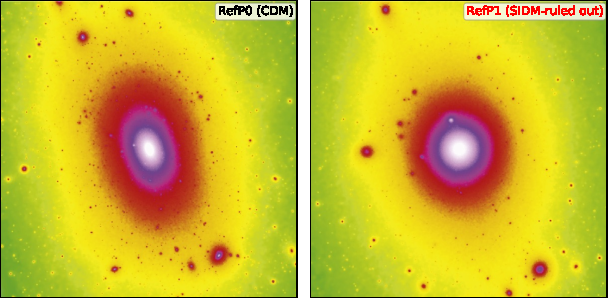
\includegraphics[width=\textwidth]{halo}}
    
    \caption{\label{fig:halo} Projected density on a \SI{270}{kpc} cube of the
    simulation of a Milky Way-like non-relativistic dark matter halo (``cold''
    dark matter, CDM). Left panel: non-interacting dark matter. Right panel:
    self-interacting dark matter (SIDM) with cross section/particle mass ratio
    \SI{10}{cm^2/g}. From \cite[21]{tulin2018}, originally from
    \cite[6]{vogelsberger2012}.}
    
\end{figure}

Where the ``Landau's arrow'' is Bayes' theorem. If the reader knows a bit about
astronomy, she may have noticed that my explanation was, to put it charitably,
qualitative. Elliptical galaxies do exist, are found in sizes smaller to larger
than the Milky Way, and possibly with low eccentricity. Furthermore,
simulations of the formation of the dark matter halo show that it actually ends
up more spherical if it \emph{does} interact, see \autoref{fig:halo}, and that
it has a rich substructure. Dark matter is expected to form aggregations of all
sizes down to the mass of the Earth \cite[1]{vogelsberger2012}.

To rule out the possibility of dark matter solar systems and planets etc.,
I~have to invoke actual measurements. In~2006 an analysis of a pair of
colliding clusters of galaxies \cite{clowe2006}, where the smaller one is named
``Bullet cluster'', showed with high confidence that the barycenters of the two
clusters have passed through, following the galaxies, while the intergalactic
gas clouds, visible in X-rays, bumped into each other. The clouds are about ten
times more massive than the galaxies, so the observed motion of the barycenters
is a strong evidence of the presence of heavy, invisible and collisionless
haloes associated to the clusters. See \autoref{fig:bullet}.

Looking at thirty such collisions, \cite{harvey2015} obtains a \SI{95}\%
confidence level upper bound on the cross section/particle mass ratio of
$\SI{0.47}{cm^2/g} = \SI{0.84}{barn/GeV}$. The limit is on the ratio, instead
of just the cross section, because the total mass is fixed by the lensing
measurement, and the mass of individual dark matter particles is unknown, and
could vary by many orders of magnitude \cite[474]{zyla2020}. This is about the
same ratio of a nucleon: cross section $\sim\SI{1}{barn}$, mass \SI{1}{GeV}.
An atom has the same mass, but cross section $10^{10}$ times higher, so
definitely dark matter is not forming anything similar to us unless we seek
very far-fetched speculations.

\begin{figure}
    
    \widecenter{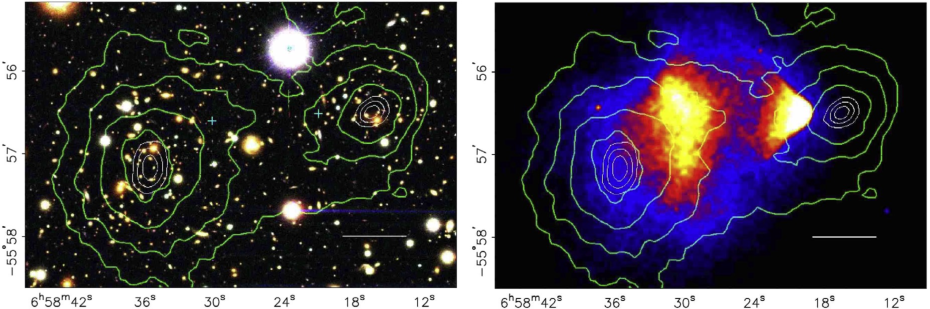
\includegraphics[width=1.3\textwidth]{bullet}}
    
    \caption{\label{fig:bullet} Left panel: photo of the Bullet cluster and its
    companion in the optical band. Right panel: the same patch of sky in
    X-rays, where the intergalactic gas is visible. The contours represent the
    mass density obtained from gravitational lensing. From
    \cite[29]{tulin2018}, originally from \cite[3]{clowe2006}.}
    
\end{figure}

The density of dark matter in the neighborhood of the solar system can be
inferred from its effect on the motion of nearby stars, which is measured
precisely. The most recent estimate, done with the Gaia satellite data, gives
$\sim\SI1{GeV/cm^3}$ \cite{buch2019}. For comparison, the solar wind density
at the Earth orbit is some particles per~\si{cm^3}. So to have a concrete
picture in our mind we can imagine dark matter as a cloud of stable neutrons
which does not interact with ordinary matter, and with density similar to the
solar wind. The same article informs us that whether self-interacting dark
matter would form a disk is still under debate, so my improvised speculations
were not too far off the mark. Assuming that it would, they put a limit on
the fraction of self-interacting dark matter in the halo to less than~\SI1\%.

Are there any other cool things that dark matter could do, beyond parallel
worlds? I once wondered whether it would form black holes. Black holes are
thought to originate from the cores of stars and galaxies, so definitely they
involve a lot of friction to accumulate stuff in one single place until it
collapses. But a totally non-interacting matter could form a black hole through
another venue: if by coincidence a sufficient amount of fluid passes through
one point, the density can get above the critical level necessary to form a
black hole. There is no classical lower limit to the size of a black hole,
since the Schwarzschild radius is proportional to the mass.

It turns out that, given the dark matter density, this is unlikely enough to be
considered impossible. I know this because a guy at the Kavli Institute told me
so. I could not find the paper searching on the net because, when I query
``dark matter black hole'', I am swamped by a swarm of results on the
primordial black holes (PBH). They are hypothesized small black holes formed
during the big bang that could make up all or part of the dark matter. Their
mass is constrained to be less than about five solar masses, or the effect of
their individual attraction would be visible. They are a viable hypothesis for
dark matter, although under debate \cite[485]{zyla2020}.

\section{Experimental evidence}

The Bullet cluster is currently one of the most important evidences of dark
matter, since it excludes that the observed gravitational effects could be due
to a simple modification of the gravitational laws instead of the presence of
additional unseen matter. Indeed, also the very first evidence was obtained
from galaxy clusters, by \cite{zwicky1933}. He observed that in the Coma
cluster the velocity of galaxies is much higher that what would be predicted
by applying the virial theorem with the masses obtained from the expected mass
to light ratio.

As in the case of the Bullet cluster, mass excesses are also observed with
gravitational lensing. Another clear effect is the orbital speed of stars in
the galaxies. Applying Gauss' theorem, since most of the light-emitting mass
of a galaxy is concentrated in the bulge, the orbital speed should fall off
like $1/\sqrt r$. Instead, $v(r)$ rises in the bulge and then stabilizes to an
almost constant value, indicating the presence of a halo.

The other line of evidence is cosmological. The density of matter is clearly
very inhomogeneous, with aggregation at all scales. The variations of density
at the last scattering epoch correspond to the temperature anisotropies of the
cosmic microwave background (CMB), shown in \autoref{fig:planckcmb}, which are
$\sim10^{-5}$. It is predicted that the variations would increase linearly with
the scale factor of the expansion of the universe, which from the origin of the
CMB is $\approx1100$, giving a still very small factor of $10^{-2}$ nowadays.
The additional aggregation can be explained by a pre-existing matter which was
already decoupled from radiation. Moreover, the presence of this matter
directly influences the angular spectrum of the CMB, which is given by
stochastic collapse-compression-expansion cycles in the primordial plasma, and
from which it is determined that dark matter amounts to \SI{85}\% of the total
matter density of the universe. This value agrees with the gravitational
observations.

\begin{figure}
    
    \widecenter{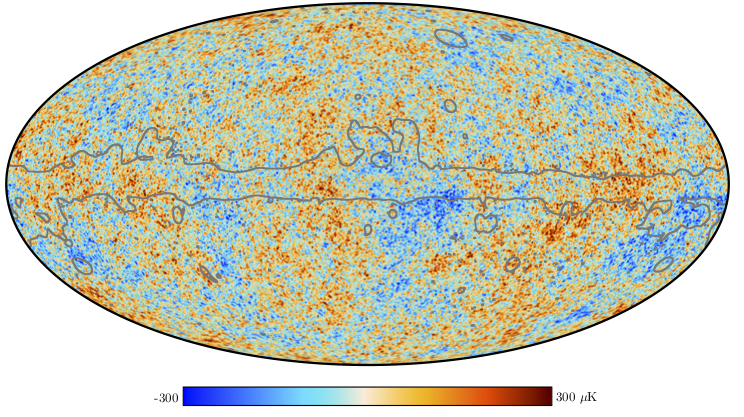
\includegraphics[width=\textwidth]{planckcmb}}
    
    \caption{\label{fig:planckcmb} Map of the variation of temperature of the
    cosmic microwave background (CMB) relative to the mean \SI{2.73}{K} and to
    the Doppler shift caused by our motion relative to the CMB. From the 2018
    Planck release \cite[fig.~6]{aghanim2020}.}
    
\end{figure}

\section{Direct detection}

All models of dark matter, apart from modified gravitational theories and
primordial black holes, postulate that dark matter is constituted by
unclassified particles. Neutrinos do behave like dark matter and account in
some part for it, but they are estimated to contribute only~\SI1\%. The limit
comes from the fact that, being relativistic (``hot'' dark matter), they would
not aggregate and solve the problem of the density variations. I have never
heard of models where dark matter is a continuous fluid.

Most of the experimental efforts are directed towards the detection of WIMPs,
``weakly interacting massive particles''. WIMP stand for a generic additional
particle in the Standard Model, which to predict the correct relic density of
dark matter after the cool down, would need to have a self-annihilation cross
section with an order of magnitude similar to the one expected for a particle
which interacts through the weak force, and a mass with an order of magnitude
around \SI{100}{GeV}.

Anyway, the point is hoping that dark matter scatters on electrons and nucleons
in the same way of a neutrino. Then, to leading order, the angular distribution
can be calculated independently of the details of the interaction. Assuming a
thermal distribution for the velocity of dark matter particles in the halo,
using the measured local mass density, and assuming a specific particle mass,
then the rate of scatterings in a target can be predicted, proportional to the
cross section. The lack of signals in a given time frame then puts an upper
limit on the cross section given the assumed mass.

\autoref{fig:sigmalimits} shows the limits obtained in this way by recent
experiments. Currently the most stringent constraints are set by experiments
hosted at Laboratori Nazionali del Gran Sasso (LNGS), DarkSide50 and Xenon1T.
Those limits are for spin-independent (SI) scattering. There are also
measurements that consider an interaction term with the spin (spin-dependent,
SD), but they are less sensible because the whole nucleus of the target atoms
counts for its overall spin, while with SI each nucleon contributes coherently.

From the curves it is evident that there is only a finite range of masses
probed by these searches.

The lower limit comes from the mass of the target particle. The scattering
would be detected by the recoil of the nucleus, which produces ionization and
scintillation light. If the recoil energy is too small it can not be detected,
with different thresholds depending on the detection technique, and of course
the recoil momentum goes to zero as the incoming particle mass decreases.
Considering electrons instead of nuclei, lower masses can be probed, but the
measurements are less sensitive because the radiation background of neutrons,
impacting nuclei, is kept better under control than gamma and beta rays which
impact electrons.

The upper limit is softer and comes from the fact that in this problem the mass
density of dark matter is fixed by gravitational measurements. Assuming an
higher particle mass means a proportionally lower number density, which is what
determines the rate together with the cross section, so the limits go up
linearly with the mass. In other words, the limitation is the size of the
target times the exposure time.

\begin{figure}
    
    \widecenter{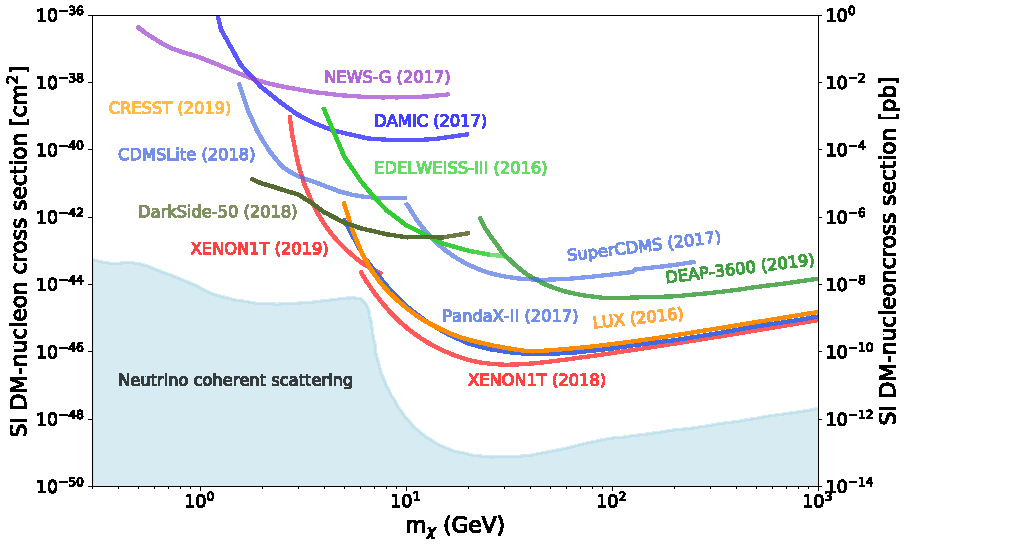
\includegraphics[width=\textwidth]{sigmalimits}}
    
    \caption{\label{fig:sigmalimits} \SI{90}\% C.L.\ upper limits on the
    WIMP-nucleon SI scattering cross section, conditional on the WIMP mass.
    From \cite[fig.~27.1 p.~481]{zyla2020}. These limits do not keep into
    account the uncertainty on the local mass and velocity distributions of
    dark matter \cite[sec.~3.1]{baxter2021}.}
    
\end{figure}

The two most popular choices for the target material are liquid argon and
xenon. Being fluid, they can be purified from radioactivity to an high degree,
more than a solid scintillator. Being noble elements, ionized electrons can
drift without producing a shower or recombining, allowing to use a time
projection chamber (TPC) to reconstruct the position, which is needed to
exclude signals near the surface, where there is additional background from the
surrounding components of the detector. Of the stable noble elements, they have
the best scintillation yield, about 40 photons per~\si{keV}.

There are other dark matter models and other kinds of experimental techniques.
At the large hadron collider (LHC), dark matter is searched through missing
energy or looking for new resonances. An interesting method is discriminating
the dark matter signal from the background using the motion of the Earth
relative to the halo, which is expected to induce a seasonal variation in the
rate and directionality of the recoils. A curious proposal of this kind
considered using RNA strands to achieve high spatial and directional resolution
\cite{drukier2015}. For a complete overview on the matter, see the particle
data group \cite[sec.~27]{zyla2020}. \cite[ch.~1]{savarese2018} gives a more
detailed introduction to some topics.
